\documentclass{article}
\usepackage[margin=1in]{geometry}
\usepackage{amsmath,amssymb}
\usepackage{booktabs}
\usepackage{float}
\usepackage{graphicx}
\usepackage{microtype}
\usepackage{tabularx}
\usepackage{xcolor}
\usepackage{xurl}
\usepackage{hyperref}

\definecolor{lanterngreen}{HTML}{176B55}
\hypersetup{
  colorlinks=true,
  linkcolor=lanterngreen,
  citecolor=lanterngreen,
  urlcolor=lanterngreen,
  pdftitle={LanternTrace: Reaction--Diffusion Physics for Predicting Spotted Lanternfly Invasion},
  pdfauthor={Alex Arthur Dils}
}
\setlength{\parindent}{0.2in}
\setlength{\parskip}{3pt}
\newcommand{\ap}{\operatorname{AP}}

\title{LanternTrace: Reaction--Diffusion Physics for Predicting Spotted Lanternfly Invasion}
\author{Alex Arthur Dils}
\date{\today}

\begin{document}
\maketitle

\begin{abstract}
\textbf{Rationale:} Understanding the advancing spotted lanternfly invasion front is important because surveillance and control are most useful before a new population becomes widely established. \textbf{Methods:} We developed Eco-RD, a reaction--diffusion model in which local growth and movement depend on climate and edible host vegetation. The model was fitted on 2019--2023 first-report data and frozen before evaluation on 2024 and 2025. \textbf{Results:} Eco-RD achieved mean average precision of 0.493, compared with 0.447 for a transferred Cook-2021 kernel, 0.343 for a transferred Ruzzier-2025 resistance-distance model, and 0.281 for distance alone. A flexible statistical covariate model remained higher at 0.511. \textbf{Conclusion:} Environmental resistance improved the selected published mechanistic baselines on this retrospective first-report task, but the model does not estimate absolute lanternfly abundance and has not yet been prospectively validated. LanternTrace provides a public, interpretable interface for examining these predictions.
\end{abstract}

\section{Introduction}

\textbf{The spotted lanternfly invasion creates a measurable agricultural and economic burden.} The insect was first detected in the United States in Berks County, Pennsylvania, in 2014, and by August 2025 some degree of infestation had been reported in 19 states and the District of Columbia---an expansion of hundreds of miles in little more than a decade \cite{usda2025}. A Penn State economic study estimated \$50.1 million in annual total economic damage in the then-current southeastern Pennsylvania quarantine zone, including \$13.1 million in direct agricultural losses. The same study projected \$324.9 million in annual statewide losses under expected damage and \$554.0 million under its worst-case scenario \cite{harper2019}. These are Pennsylvania scenario estimates, not measured national crop losses.

\textbf{Tracking the invasion front allows limited surveillance and management resources to be directed toward places where new reports are most likely.} A cumulative occurrence map shows everywhere the insect has ever been reported, but it does not directly answer where the next report will occur. That distinction matters because a prediction method can look accurate simply by assigning high risk to already established areas. We therefore define the outcome as a first report in a previously unreported grid cell.

\textbf{Climate, edible vegetation, local dispersal, wind, and human transport can all influence spotted lanternfly spread.} Temperature and moisture affect establishment and phenology \cite{wakie2020,barker2025}; tree-of-heaven, grape, walnut, maple, and willow provide hosts of differing quality \cite{nixon2020}; and human-assisted movement produces long-distance jumps that local diffusion cannot explain \cite{ladin2023}. Wind may affect short-range movement, but the frozen benchmark in this paper isolates the two environmental surfaces that were available consistently across the domain: climate and host vegetation. The application's wind display is an exploratory sensitivity layer, not part of the fitted performance claim.

\textbf{Previous spread models are informative but often emphasize distance, broad suitability, or transportation separately.} Cook and colleagues modeled invasion hazard using spatial proximity and population \cite{cook2021}. Ruzzier and colleagues combined climatic and host suitability with resistance distance and a published annual dispersal scale \cite{ruzzier2025}. PoPS incorporates local kernels and long-distance transportation processes \cite{jones2022}. These approaches establish strong precedents, but transferring any published model to a new grid, observation source, and prediction endpoint can change its performance.

\textbf{Here we present a mechanistic model and a machine-learning alternative that learn from known drivers without treating the observed range as the answer.} Eco-RD solves a reaction--diffusion update in which climate and edible host vegetation jointly control both establishment and resistance to movement. In parallel, OG-RDE fits a regularized statistical hazard using multiscale frontier, environmental, geographic, and simulated-physics features. The mechanistic model is intended to remain interpretable at the level of a single cell; the learned model asks how much predictive signal remains when those assumptions are relaxed.

\textbf{We evaluate the models on held-out 2024--2025 first reports and make the results publicly inspectable.} Model parameters were selected using only 2019--2023 outcomes and then frozen. The 2026 records are incomplete and are therefore reported only as interim monitoring, not as a complete holdout. The interactive application is available at \href{https://www.alex-dils.com/lanterntrace/app/}{alex-dils.com/lanterntrace/app}.

\section{Methods}

\subsection{Occurrence data}

\textbf{Spotted lanternfly occurrence records were obtained from a locked GBIF snapshot rather than directly from iNaturalist.} The snapshot, retrieved on August 2, 2026, contains 62,791 public-coordinate records; 57,999 dated records fall inside the United States analysis mask \cite{gbif}. GBIF aggregates multiple publishers and citizen-science sources, which preserves a reproducible record key and source trail. The records collapse to 2,484 unique cell-years and 675 unique first-report cells. Because these are opportunistic reports, an unreported cell is a pseudo-absence: it can be uninvaded, invaded but undetected, or detected but not yet published.

\subsection{Adding cells to the map}

\textbf{The map divides the northeastern United States into a fixed $0.2^\circ$ grid.} The $50\times70$ domain spans $37$--$47^\circ$N and $82$--$68^\circ$W. A 2025 U.S. Census state boundary mask leaves 1,652 eligible land cells; at the center of the domain, one cell is approximately 22 km north--south by 16 km east--west. Cells whose centers fall outside the U.S. land mask are excluded from fitting and evaluation. For each eligible cell $i$, the first-report year $T_i$ is the earliest dated occurrence. The target for year $t$ is
\begin{equation}
  y_{i,t}=\mathbb{1}(T_i=t), \qquad
  i\in\mathcal{E}_t=\{i:T_i\geq t,\ L_i=1\},
\end{equation}
where $L_i$ is the land mask. Thus, every candidate was unreported at the forecast origin.

\begin{figure}[htbp]
  \centering
  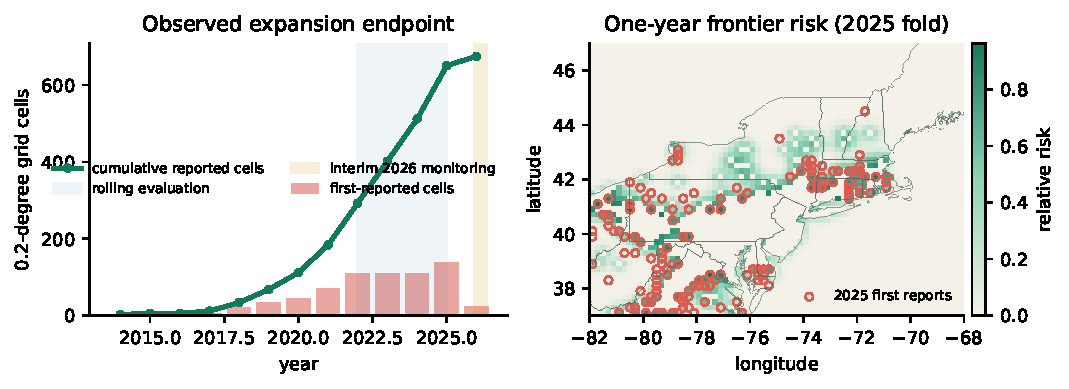
\includegraphics[width=\textwidth]{../figures/fig1_endpoint_and_map.pdf}
  \caption{Study endpoint and analysis grid. Left, cumulative reported cells compared with the smaller first-report endpoint. Right, the frozen 2025 Eco-RD risk surface, new reports, U.S. boundaries, and masked cells. The modeled field is relative risk, not abundance.}
  \label{fig:endpoint}
\end{figure}

\subsection{Population standardization}

\textbf{Population standardization is used to make the observed-report display less sensitive to where more people are available to report insects.} For the interactive observed layer, cumulative reports in a cell are converted to reports per 100,000 residents and stabilized toward the national rate with an empirical-Bayes population prior. Neighboring cells are then smoothed to reduce visually abrupt sampling gaps. This display should be interpreted as a relative population-adjusted reporting signal. Population normalization is deliberately \emph{not} applied to the first-report labels or to the Eco-RD state, because dividing the binary outcome by population would change the forecast question and could make sparsely populated cells artificially extreme.

\subsection{Climate and host vegetation}

\textbf{Climate suitability combines temperature and moisture variables associated with spotted lanternfly establishment.} The surface uses WorldClim 2 BIO1, BIO3, BIO9, and BIO19 variables \cite{worldclim}, selected to represent annual temperature, temperature evenness, dry-quarter temperature, and cold-quarter precipitation in line with published establishment analyses \cite{wakie2020}. The resulting score $C_i\in[0,1]$ is a relative suitability index.

\textbf{Vegetation suitability represents plants that spotted lanternflies can eat rather than generic greenness.} We assembled a locked GBIF host snapshot containing 3,600 public-coordinate records for each of six host groups: tree-of-heaven, \textit{Vitis} species, black walnut, silver maple, \textit{Salix} species, and red maple. Each taxon was gridded, smoothed, log transformed, and normalized independently before combination. The combination weights are controlled-experiment mean first-instar survival days reported by Nixon and colleagues \cite{nixon2020}. The resulting score $V_i\in[0,1]$ is a host-availability proxy, not a remotely sensed biomass measurement.

\begin{table}[htbp]
\centering
\caption{Model quantities, values, and evidential status. Biological and transferred-model constants are linked to literature; fitted and numerical terms are labeled separately.}
\label{tab:parameters}
\small
\begin{tabularx}{\textwidth}{@{}l l X@{}}
\toprule
Quantity & Value & Basis and interpretation \\
\midrule
Tree-of-heaven survival & 72.5 d & Experimental host weight \cite{nixon2020} \\
Wild grape survival & 63.9 d & Experimental host weight \cite{nixon2020} \\
Black walnut survival & 62.9 d & Experimental host weight \cite{nixon2020} \\
Silver maple survival & 58.0 d & Experimental host weight \cite{nixon2020} \\
Willow survival & 47.0 d & Experimental host weight \cite{nixon2020} \\
Red maple survival & 22.2 d & Experimental host weight \cite{nixon2020} \\
Cook distance decay & 0.045 km$^{-1}$ & Published county-scale kernel \cite{cook2021} \\
Ruzzier annual distance & 25.418 km & Published 99th-percentile dispersal scale \cite{ruzzier2025} \\
Ruzzier resistance $k,x_0$ & 15, 0.5 & Published logistic resistance transform \cite{ruzzier2025} \\
Eco-RD diffusion $D$ & 0.28 month$^{-1}$ & Selected on 2019--2023 first reports \\
Eco-RD growth $r$ & 0.24 month$^{-1}$ & Selected on 2019--2023 first reports \\
Host/climate powers & 1.0, 1.6 & Selected on 2019--2023 first reports \\
Minimum conductivity & 0.08 & Numerical floor; prevents false hard barriers \\
Grid and time step & $0.2^\circ$, 1 month & Numerical design; not a biological constant \\
\bottomrule
\end{tabularx}
\end{table}

\subsection{Resistance in a single cell}

\textbf{A cell's resistance is the inverse of how easily invasion pressure can move through its climate--vegetation environment.} First, the two environmental scores are combined as
\begin{equation}
S_i=\sqrt{
  [f_V+(1-f_V)V_i]^{p_V}
  [f_C+(1-f_C)C_i]^{p_C}},
\end{equation}
where $S_i$ is establishment suitability, $f_V$ and $f_C$ are optional floors, and $p_V$ and $p_C$ control how strongly intermediate vegetation and climate values are penalized. The geometric mean requires both factors to be favorable: good vegetation cannot fully compensate for unsuitable climate, and favorable climate cannot compensate for the absence of hosts.

\textbf{Suitability becomes movement conductivity through $k_i=L_i(0.08+0.92S_i)$ and resistance through $R_i=1/k_i$.} An ideal land cell has $S_i=1$, $k_i=1$, and $R_i=1$. A very poor land cell approaches $k_i=0.08$ and $R_i=12.5$, meaning that movement is much slower but not declared impossible. A masked water or non-U.S. cell has $L_i=0$ and cannot carry pressure. Across an edge, the model uses the harmonic mean of the two conductivities, so one highly resistant cell slows exchange in both directions.

\subsection{Reaction--diffusion model}

\textbf{Eco-RD updates relative invasion pressure through environment-dependent diffusion and logistic establishment.} Let $u_i^n\in[0,1]$ be the relative pressure in cell $i$ at monthly step $n$. The discrete update is
\begin{equation}
u_i^{n+1}=\Pi_{[0,1]}\left[
u_i^n+D\,\nabla_h\!\cdot(k\nabla_h u^n)_i
+rS_i u_i^n(1-u_i^n)
\right].
\end{equation}
The first term preserves the existing state. The second spreads pressure between neighboring cells, slowed by conductivity $k$. The third allows local establishment, scaled by suitability $S_i$, with logistic saturation preventing unbounded growth. The projection $\Pi_{[0,1]}$ keeps the numerical state within its declared range. The state $u_i$ is a ranking signal; it is not an estimated number of insects.

\textbf{Smaller visual cells do not create new ecological evidence.} The scientific benchmark is solved at the fixed $0.2^\circ$ resolution so every model is compared on the same support. The application may subdivide or interpolate cells for smoother viewing, but those subcells inherit the parent solution unless the inputs and PDE are refitted at the finer grid. A genuine higher-resolution physics study would require higher-resolution host, climate, occurrence, and population inputs together with a new convergence analysis.

\subsection{Parameter fitting and comparison models}

\textbf{Eco-RD parameters were selected before the holdout period by exhaustive search.} We evaluated 972 combinations of diffusion, growth, environmental floors, and environmental powers. Selection maximized mean annual average precision on 2019--2023 first-report targets, with worst-year performance as the tie breaker. The selected values were $D=0.28$, $r=0.24$, $f_V=f_C=0$, $p_V=1.0$, and $p_C=1.6$. No 2024 or 2025 label entered the search.

\textbf{The comparison set separates distance, published mechanistic forms, and a flexible statistical control.} Distance-only ranks cells by proximity to the previously reported range. The Cook-2021 comparator transfers the published $\exp(-0.045d)$ spatial kernel to grid-cell centers \cite{cook2021}. The Ruzzier-2025 comparator transfers the published suitability-to-resistance transform and 25.418-km annual distance scale \cite{ruzzier2025}. Fisher--KPP uses uniform land conductivity and growth. The covariate hazard is a regularized logistic model using multiscale frontier, climate, host, geographic, and terrain predictors. OG-RDE additionally includes reaction--diffusion state fields. These transfers are fair common-endpoint tests, not exact replications of the original studies.

\begin{figure}[H]
  \centering
  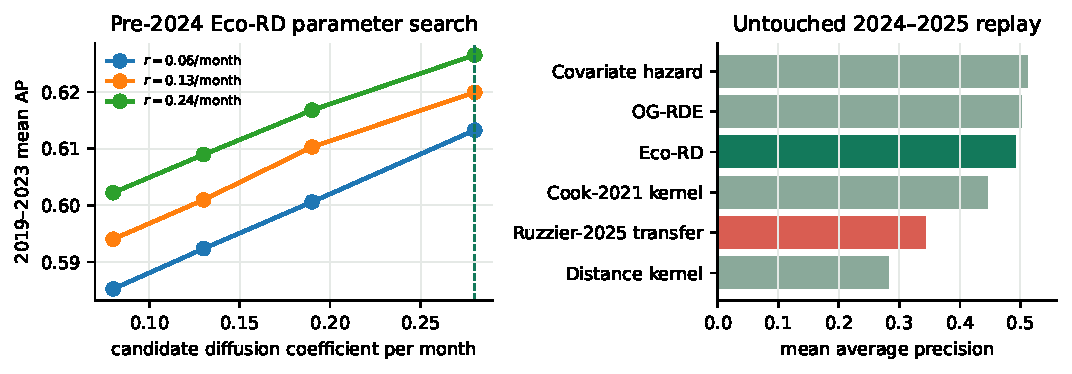
\includegraphics[width=0.82\textwidth]{../figures/fig9_eco_rd_fit.pdf}
  \caption{Eco-RD parameter fitting and untouched evaluation. Left, the pre-2024 search surface after retaining the best environmental settings for each diffusion--growth pair. Right, mean average precision on 2024--2025 after the specification was frozen.}
  \label{fig:fit}
\end{figure}

\subsection{Evaluation}

\textbf{Evaluation ranks only cells that had not been reported before each target year.} Average precision (AP) is primary because new reports are rare relative to candidate cells. AP summarizes precision across all recall thresholds. We also report recall among the highest-ranked 5\% of eligible cells, representing a constrained survey budget. The frozen evaluation contains 110 positive cells among 1,250 candidates in 2024 and 139 positives among 1,140 candidates in 2025.

\textbf{Spatial uncertainty was assessed with geographic blocks rather than random point splits.} The domain was partitioned into fixed $2^\circ\times2^\circ$ blocks, and 2,500 block-bootstrap samples preserved all repeated years within a sampled block. Because only two untouched years are available and occurrence data are presence-only, intervals are descriptive rather than a substitute for prospective surveillance.

\section{Results}

\subsection{Fitted environmental response}

\textbf{The fitted model gave climate a stronger penalty than host vegetation.} The selected powers were $p_C=1.6$ and $p_V=1.0$, so middling climate values were reduced more strongly than middling host scores. Both fitted floors were zero, meaning that the model did not grant an artificial minimum establishment quality when either environmental factor was absent. The conductivity floor remained 0.08 for numerical continuity; it changes movement resistance but does not create local establishment where $S_i=0$.

\subsection{Frozen temporal performance}

\textbf{Eco-RD improved all three selected distance and published mechanistic baselines in both untouched years.} Eco-RD scored 0.490 AP in 2024 and 0.496 in 2025, averaging 0.493. Its mean AP was 10.4\% higher than the Cook-2021 transfer, 43.6\% higher than the Ruzzier-2025 transfer, and 75.1\% higher than distance alone. At the highest-ranked 5\% of cells, Eco-RD captured 36 of 110 new reports in 2024 and 35 of 139 in 2025.

\begin{table}[H]
\centering
\caption{Frozen 2024--2025 first-report performance. Mean R@5\% is annual recall among the highest-ranked 5\% of eligible cells.}
\label{tab:results}
\begin{tabular}{@{}lrrr@{}}
\toprule
Model & 2024 AP & 2025 AP & Mean R@5\% \\
\midrule
Covariate hazard & 0.495 & 0.527 & 0.285 \\
OG-RDE & 0.491 & 0.513 & 0.280 \\
Eco-RD & 0.490 & 0.496 & 0.290 \\
Transport RD & 0.478 & 0.482 & 0.278 \\
Climate RD & 0.469 & 0.480 & 0.253 \\
Fisher--KPP & 0.464 & 0.480 & 0.258 \\
Cook-2021 transfer & 0.435 & 0.458 & 0.234 \\
Ruzzier-2025 transfer & 0.316 & 0.370 & 0.212 \\
Distance only & 0.275 & 0.288 & 0.255 \\
\bottomrule
\end{tabular}
\end{table}

\textbf{The strongest result is therefore narrower than universal state-of-the-art superiority.} The study-built covariate hazard averaged 0.511 AP and OG-RDE averaged 0.502, both above Eco-RD. Moreover, the paired geographic-block interval for Eco-RD minus Cook was $-0.037$ to $0.033$, and the interval for Eco-RD minus Ruzzier was $-0.034$ to $0.070$. Both cross zero. The evidence supports better annual ranking than these transferred published mechanistic baselines on this endpoint, but not a uniform advantage in every region or over every statistical model.

\begin{figure}[H]
  \centering
  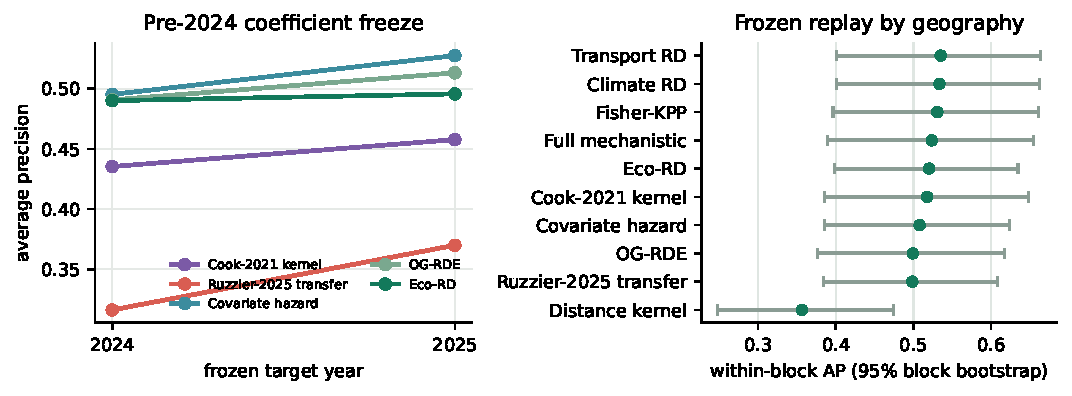
\includegraphics[width=\textwidth]{../figures/fig5_frozen_validation.pdf}
  \caption{Frozen temporal replay. Left, annual AP after coefficients and specifications were fixed through 2023. Right, within-block AP with geographic-block bootstrap intervals. Annual improvements do not imply a resolved local advantage in every block.}
  \label{fig:frozen}
\end{figure}

\subsection{Spatial pattern of predictions}

\textbf{The maps show useful concentration near the advancing front together with structured misses.} The model places high pressure around previously reported cells where host and climate conditions are favorable. Isolated first reports beyond the highest-risk contour remain difficult, consistent with unmodeled hitchhiking, uneven observation, or both. Smooth green regions are interpolated model pressure, whereas ringed points are reported evidence.

\begin{figure}[H]
  \centering
  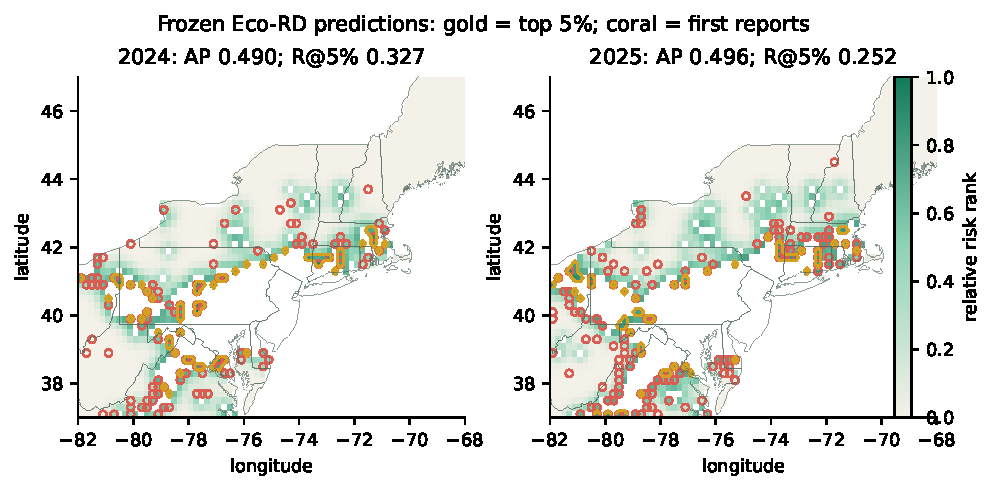
\includegraphics[width=\textwidth]{../figures/fig6_frozen_maps.pdf}
  \caption{Frozen Eco-RD predictions for 2024 and 2025. Gold contours enclose the fixed top-5\% survey allocation; coral rings identify cells first reported in that year. White cells are outside the eligible U.S. land domain.}
  \label{fig:maps}
\end{figure}

\section{Discussion}

\textbf{Adding climate and edible host vegetation improved a simple physical spread model because the invasion front is not equally likely to establish in every direction.} Distance alone assumes that all nearby cells are interchangeable. Eco-RD instead lets suitable cells both accept pressure more readily and support faster local growth, while unfavorable cells slow movement and establishment. This creates an interpretable environmental resistance surface without requiring each cell to have a separately fitted coefficient.

\textbf{The single-cell resistance definition makes the model easier to inspect but does not make the parameters directly biological.} A resistance of 12.5 means that the model's conductivity is one-twelfth-and-a-half of the ideal baseline; it does not mean that a lanternfly experiences 12.5 units of physical force or that arrival takes 12.5 years. Likewise, $D$ and $r$ are predictive coefficients at this grid and monthly time step. They cannot be converted into absolute flight speed, population growth, or insect counts without independent abundance data and calibration.

\textbf{Wind and human transport are important next mechanisms, but they require separately validated inputs.} The current public app can display average wind vectors and exploratory advection, yet the frozen claim in this paper is based on climate and host vegetation. A climatological mean wind field cannot recover the timing of individual flight events, and human transport can produce jumps unrelated to prevailing wind. Future fitting should use versioned weather reanalysis, road and rail networks, freight or traffic flows, and held-out event dates to determine whether these terms improve prediction rather than merely making the animation more realistic.

\textbf{Presence-only data remain the main limitation.} A first report is the first record available in the snapshot, not necessarily the first biological arrival. Reporting effort varies with population, publicity, agency programs, and access. The population-adjusted observed layer helps users interpret report intensity, but it cannot repair the forecast labels. Structured trap or inspection data with documented effort are needed to separate occupancy from detection and to calibrate probabilities.

\textbf{The frozen replay improves temporal separation but is not a preregistered prospective test.} The 2024--2025 labels did not fit the model, yet the overall analysis was designed after the 2026 snapshot existed, and later uploads can populate earlier event years. Only two complete untouched years are available. A stronger study would publish a fixed 2027 risk map before outcomes accrue, retain the complete versioned input bundle, and evaluate against independent survey effort.

\textbf{The economic figures motivate prioritization but should not be read as LanternTrace forecasts.} The Penn State values are scenario-based estimates for Pennsylvania agriculture, forestry, and the wider economy in 2019 conditions \cite{harper2019}. LanternTrace does not presently convert modeled pressure into crop-specific yield loss or dollars. A defensible economic extension would couple calibrated occupancy and abundance to crop exposure, damage functions, prices, and uncertainty intervals.

\section{Conclusion}

\textbf{LanternTrace moves spotted lanternfly prediction from a distance-only front toward an interpretable environmental spread model.} Eco-RD combines climate and edible host vegetation in a reaction--diffusion equation, fits six parameters before the holdout period, and ranks only cells that were previously unreported. On the frozen 2024--2025 replay, the model improved mean AP by 10.4\% over the transferred Cook-2021 kernel, 43.6\% over the transferred Ruzzier-2025 resistance-distance form, and 75.1\% over distance alone.

\textbf{The model is best understood as a transparent search-prioritization tool rather than a count forecast.} It does not estimate the number of lanternflies in a cell, its geographic intervals do not establish uniform superiority, and a flexible statistical control remains stronger. Prospective evaluation with documented survey effort, event-specific weather, and transportation data is the next step toward a more informed and defensible invasion digital twin.

\section*{Data and code availability}

The source code, locked-input manifests, generated tables, figures, tests, and application are available in the \href{https://github.com/axel-slid/lanterntrace-explorer}{public project repository}. The \href{https://www.alex-dils.com/lanterntrace/app/}{interactive LanternTrace map} is also publicly available. Third-party data retain their original licenses. A permanent archive DOI and GBIF derived-dataset DOI remain release tasks.

{\footnotesize
\begin{thebibliography}{12}
\setlength{\itemsep}{0pt}

\bibitem{usda2025}
U.S. Department of Agriculture Animal and Plant Health Inspection Service.
Spotted Lanternfly: Current Status.
Updated August 26, 2025.
\href{https://www.aphis.usda.gov/plant-pests-diseases/slf}{USDA APHIS}.

\bibitem{harper2019}
Harper, J.K., Stone, W., Kelsey, T.W., and Kime, L.F. (2019).
\textit{Potential Economic Impact of the Spotted Lanternfly on Agriculture and Forestry in Pennsylvania}.
Pennsylvania State University and Center for Rural Pennsylvania.
\href{https://aese.psu.edu/research/centers/cecd/publications/economic-analyses-including-covid-19-analysis/economic-impact/spotted-lanternfly-2019.pdf/view}{Penn State report}.

\bibitem{wakie2020}
Wakie, T.T. et al. (2020).
Establishment risk of \textit{Lycorma delicatula} in the United States and globally.
\textit{Journal of Economic Entomology} 113, 306--314.
\href{https://doi.org/10.1093/jee/toz259}{doi:10.1093/jee/toz259}.

\bibitem{barker2025}
Barker, B.S., Beyer, J., and Coop, L. (2025).
Real-time integrative mapping of phenology and climatic suitability for the spotted lanternfly.
\textit{Insects} 16, 790.
\href{https://doi.org/10.3390/insects16080790}{doi:10.3390/insects16080790}.

\bibitem{nixon2020}
Nixon, L.J. et al. (2020).
Distribution, survival, and development of spotted lanternfly on host plants found in North America.
\textit{Environmental Entomology} 49, 1270--1281.
\href{https://doi.org/10.1093/ee/nvaa126}{doi:10.1093/ee/nvaa126}.

\bibitem{ladin2023}
Ladin, Z.S. et al. (2023).
Human-mediated dispersal drives the spread of the spotted lanternfly.
\textit{Scientific Reports} 13, 1098.
\href{https://doi.org/10.1038/s41598-022-25989-3}{doi:10.1038/s41598-022-25989-3}.

\bibitem{cook2021}
Cook, R.T. et al. (2021).
Spatial dynamics of spotted lanternfly invasion in the northeastern United States.
\textit{NeoBiota} 70, 23--42.
\href{https://doi.org/10.3897/neobiota.70.67950}{doi:10.3897/neobiota.70.67950}.

\bibitem{ruzzier2025}
Ruzzier, E. et al. (2025).
Predicting the global distribution and invasion scenarios of the spotted lanternfly, \textit{Lycorma delicatula}.
\textit{NeoBiota} 103, 267--298.
\href{https://doi.org/10.3897/neobiota.103.154246}{doi:10.3897/neobiota.103.154246}.

\bibitem{jones2022}
Jones, C. et al. (2022).
Spotted lanternfly predicted to establish in California by 2033 without preventative management.
\textit{Communications Biology} 5, 558.
\href{https://doi.org/10.1038/s42003-022-03447-0}{doi:10.1038/s42003-022-03447-0}.

\bibitem{worldclim}
Fick, S.E. and Hijmans, R.J. (2017).
WorldClim 2: new 1-km spatial climate surfaces for global land areas.
\textit{International Journal of Climatology} 37, 4302--4315.
\href{https://doi.org/10.1002/joc.5086}{doi:10.1002/joc.5086}.

\bibitem{gbif}
GBIF.org (2026).
\textit{Lycorma delicatula} occurrence API snapshot, retrieved August 2, 2026; included record keys and checksums archived with this study.
\url{https://www.gbif.org/species/5157899}.

\end{thebibliography}
}

\end{document}
